\documentclass[tikz,border=3mm]{standalone}
\usetikzlibrary{arrows.meta,shapes.geometric}

\tikzset{
    mynode/.style={circle,draw,inner sep=2pt},
    myarrow/.style={->,thick,-Stealth}
}

\begin{document}
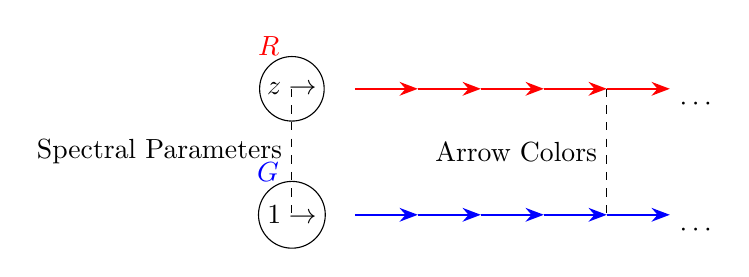
\begin{tikzpicture}[scale=0.8]
    % Nodes for z -> and 1 ->
    \node[mynode] (z) at (-4,2) {$z \to$};
    \node[mynode] (one) at (-4,0) {$1 \to$};

    % Arrow labels above the nodes
    \node[above] at (z.north west) {$\textcolor{red}{R}$};
    \node[above] at (one.north west) {$\textcolor{blue}{G}$};

    % Horizontal arrows
    \foreach \x in {-3,-2,...,1} {
        \draw[myarrow,color=red] (\x,2) -- ++(1,0);
        \draw[myarrow,color=blue] (\x,0) -- ++(1,0);
    }

    % Ellipsis to indicate infinity
    \node[below right] at (2,2) {\(\bm{\cdots}\)};
    \node[below right] at (2,0) {\(\bm{\cdots}\)};

    % Vertical lines to separate different parts
    \draw[dashed] (-4,2) -- (-4,0);
    \draw[dashed] (1,2) -- (1,0);

    % Labels for the vertical lines
    \node[left] at (-4,1) {Spectral Parameters};
    \node[left] at (1,1) {Arrow Colors};
\end{tikzpicture}
\end{document}